\documentclass[]{beamer} %zaradi [handout] \pause ne dela
\usepackage[T1]{fontenc}
\usepackage[utf8]{inputenc}
\usepackage[slovene]{babel}
\usepackage{pgfpages}
\usepackage{amsmath}
\usepackage{amssymb}
\usepackage{colortbl}
\usepackage{tikz}
\usepackage{array}
\usepackage{amsmath,amssymb,amsfonts,amsthm}
\usepackage{mathtools}
\usepackage{dsfont}
\usepackage{xcolor}

\setbeameroption{hide notes}
%\setbeameroption{show notes on second screen=right}

\mode<presentation>
\usetheme{Berlin}
\useinnertheme[shadows]{rounded}
\useoutertheme{infolines}
\usecolortheme{spruce}
\usepackage{palatino}
\usefonttheme{serif}

%okolja za izreke, definicije, ...
\theoremstyle{plain}
\newtheorem{izrek}{Izrek}
\newtheorem{definicija}{Definicija}
\newtheorem{trditev}{Trditev}
\newtheorem{posledica}{Posledica}
\newtheorem{opomba}{Opomba}
\newtheorem{zgled}{Zgled}
\newtheorem{lema}{Lema}

%Math operators
\newcommand{\R}{\mathbb{R}}
\newcommand{\N}{\mathbb{N}}
\newcommand{\E}{\mathbb{E}}
\newcommand{\F}{\mathcal{F}}
\newcommand{\B}{\mathcal{B}}
\newcommand{\Prob}{\mathbb{P}}
\newcommand{\Pois}[1]{\text{Pois}(#1)}
\newcommand{\Var}[1]{\text{$\mathbb{V}\!\mathrm{ar}$}\left[#1\right]}
\DeclareMathOperator{\HPP}{HPP}
\DeclareMathOperator{\CPP}{CPP}

% Barve za okolja
\BeforeBeginEnvironment{definicija}{%
    \setbeamercolor{block title}{fg=black,bg=orange!40!white}
    \setbeamercolor{block body}{fg=black, bg=orange!20!white}
}
%\AfterEndEnvironment{definicija}{
% \setbeamercolor{block title}{use=structure,fg=structure.fg,bg=structure.fg!20!bg}
% \setbeamercolor{block body}{parent=normal text,use=block title,bg=block title.bg!50!bg, fg=black}
%}
\definecolor{redO}{HTML}{ea410f}
\BeforeBeginEnvironment{izrek}{%
    \setbeamercolor{block title}{fg=black,bg=redO!50!white}
    \setbeamercolor{block body}{fg=black, bg=redO!20!white}
}
\BeforeBeginEnvironment{lema}{%
    \setbeamercolor{block title}{fg=black,bg=orange!40!white}
    \setbeamercolor{block body}{fg=black, bg=orange!20!white}
}
\definecolor{blueO}{HTML}{14baeb}
\BeforeBeginEnvironment{trditev}{%
    \setbeamercolor{block title}{fg=black,bg=blueO!40!white}
    \setbeamercolor{block body}{fg=black, bg=blueO!20!white}
}
\definecolor{greenO}{HTML}{13bf54}
\BeforeBeginEnvironment{zgled}{%
    \setbeamercolor{block title}{fg=black,bg=greenO!40!white} 
    \setbeamercolor{block body}{fg=black, bg=greenO!20!white}
}

% New itemize environment bullet point
\setbeamertemplate{itemize item}{$\circ$}

%\beamertemplatenavigationsymbolsempty
\setbeamertemplate{headline}{}
%\setbeamertemplate{footline}{}

\title[CPP in njegova uporaba v financah]{Sestavljeni Poissonov proces in njegova upraba v financah}
\subtitle{}
\author[Anej Rozman]{\textbf{Anej Rozman} \\ \footnotesize Mentor: doc.~dr.~Martin Raič}
\institute[UL-FMF]{Univerza v Ljubljani, Fakulteta za matematiko in fiziko}
\date[]{}


\begin{document}

%-------------------------------------------TITLE--------------------------------------------------%
\frame{\titlepage}


%-----------------------------------------FRAME 1--------------------------------------------------%
\begin{frame}
  \frametitle{Sestavljena Poissonova porazdelitev}
  \begin{definicija}
    Naj bo $N\sim \Pois{\lambda}$  za $\lambda >0$ in $X_1, X_2, \dots$ zaporedje neodvisnih (med seboj in od $N$)
    enako porazdeljenih slučajnih spremenljivk. Potem pravimo, da ima slu"cajna spremenljivka
    \begin{equation*}
        S = \sum_{i=1}^NX_i
    \end{equation*}
    \textit{sestavljeno Poissonovo porazdelitev}. 
    \label{def:sestavljenaPoissonovaPorazdelitev}
  \end{definicija}
\end{frame}

%-----------------------------------------FRAME 2--------------------------------------------------%
\begin{frame}
  \frametitle{Karakteristi"cna funkcija}
  \begin{trditev}
    Karakteristi"cna funkcija slu"cajne vsote $S=\sum_{i = 1}^{N}X_i$ ima obliko 
    \begin{equation*}
        \varphi_{S}(u) = e^{\lambda \left(\varphi_{X_1}(u) - 1\right)}.
    \end{equation*}
    Lahko jo izrazimo kot kompozitum rodovne funkcije $G_N$ in karakteristi"cne funkcije $\varphi_{X_1}$
    \begin{align*}
      \varphi_{S}(u) = G_{N}\left(\varphi_{X_1}(u)\right).
  \end{align*}
    \label{pos:RodovnaKarakteristicna}
  \end{trditev}
\end{frame}
 
%-----------------------------------------FRAME 3--------------------------------------------------%
\begin{frame}
  \frametitle{Sestavljena Poissonova porazdelitev}
  \begin{align*}
    F_{S}(x) = \Prob\bigl(S \leq x\bigr) 
    &= \sum_{k=0}^\infty \Prob\bigl(S \leq x \mid N = k\bigr)\Prob\bigl(N = k\bigr) \\
    &= \sum_{k=0}^\infty \Prob\bigl(S_k \leq x\bigr)\Prob\bigl(N = k\bigr) \\
    &= \sum_{k=0}^\infty F_{X_1}^{*k}(x) \frac{\lambda^k}{k!} e^{-\lambda}
  \end{align*}
\end{frame}

%-----------------------------------------FRAME 4--------------------------------------------------%
\begin{frame}
  \frametitle{Sestavljena Poissonova porazdelitev}
  \begin{zgled}
        Naj bodo $X_1, X_2, \dots$ porazdeljene kot
        \begin{equation*}
            X_1\sim\text{Exp}(\mu),\quad \text{torej z gostoto} \quad  f_{X_1}(x) = \mu e^{-\mu x}; \quad x>0, \mu > 0,
        \end{equation*}
        $k$-ta 
        konvolucija porazdelitve $X_1$ je porazdelitev $\text{Gamma}(k, \mu)$.
        \begin{equation*}
            f_{X_1 + \cdots + X_k}(x) = \frac{1}{\Gamma(k)}\mu^kx^{k-1}e^{-\mu x}; \quad x>0.
        \end{equation*}
        Za $s>0$ velja
        \begin{align*}
            F_{S}(s) 
            &= \int_0^s\underbrace{\sum_{k=0}^\infty \frac{1}{(k-1)!k!}(\mu\lambda)^kx^{k-1}e^{-(\mu x + \lambda)}}_{f_S(x)}dx.
        \end{align*}
  \end{zgled}
\end{frame}

%-----------------------------------------FRAME --------------------------------------------------%

\begin{frame}
  \frametitle{Homogeni Poissonov proces ($\HPP$)}
  \begin{definicija}
    Naj bo $\lambda > 0$. Slučajnemu procesu $(N_t)_{t\geq 0}$, definiranem na verjetnostnem 
    prostoru $(\Omega, \mathcal{F}, \mathbb{P})$ in z vrednostmi v $\mathbb{N}_0$, pravimo 
    \textit{homogeni Poissonov proces} z intenzivnostjo $\lambda$, če zadošča naslednjim pogojem:
    \begin{itemize}
        \item $N_0 = 0$ \ $\Prob$-skoraj gotovo.
        \item $(N_t)_{t\geq 0}$ ima neodvisne in stacionarne prirastke,
        \item Za $0 \leq s < t$ velja $ N_t - N_s \sim\Pois{\lambda(t - s)}$,
    \end{itemize}
  \end{definicija}
\end{frame}

%-----------------------------------------FRAME --------------------------------------------------%
\begin{frame}
  \frametitle{Sestavljeni Poissonov proces ($\CPP$)}
  \begin{definicija}
    Naj bo $(N_t)_{t\geq0}$ homogeni Poissonov proces z intenzivnostjo $\lambda$. 
    Naj bo $(X_i)_{i\geq1}$ zaporedje neodvisnih (med sabo in od procesa $(N_t)_{t\geq0}$) in enako 
    porazdeljenih slučajnih spremenljivk. Potem je 
    \textit{sestavljeni Poissonov proces} $(S_t)_{t\geq0}$ definiran kot dru"zina
    slu"cajnih spremenljivk
    $$
        S_t = \sum_{i=1}^{N_t} X_i, \quad t\geq0.
    $$
    \label{def:CPP}
  \end{definicija}
\end{frame}

%-----------------------------------------FRAME --------------------------------------------------%	
\begin{frame}
  \frametitle{Sestavljeni Poissonov proces}
  \begin{trditev}
    $\CPP$ ima neodvisne in stacionarne prirastke.
  \end{trditev}
  \pause
  \begin{trditev}
    Naj bo $(S_t)_{t\geq 0}$ $\CPP$ in naj bosta $\mu = \mathbb{E}\left[X_i\right] < \infty$ 
    pri"cakovana vrednost in $\sigma^2= \Var{X_i} <\infty$ varianca
    slu"cajnih spremenljivk $X_i$. Potem sta za $t\geq0$ pri"cakovana vrednost in 
    varianca $S_t$ enaki 
    \begin{equation*}
        \E\left[S_t\right] = \mu\lambda t \qquad \text{in} \qquad \Var{S_t} = \lambda t\left(\sigma^2 + \mu^2\right).
    \end{equation*}
    \label{trd:PricVarCPP}
  \end{trditev}
\end{frame}

%-----------------------------------------FRAME --------------------------------------------------%
\begin{frame}
  \frametitle{Sestavljeni Poissonov proces}
  \begin{figure}[H]
    \centering
    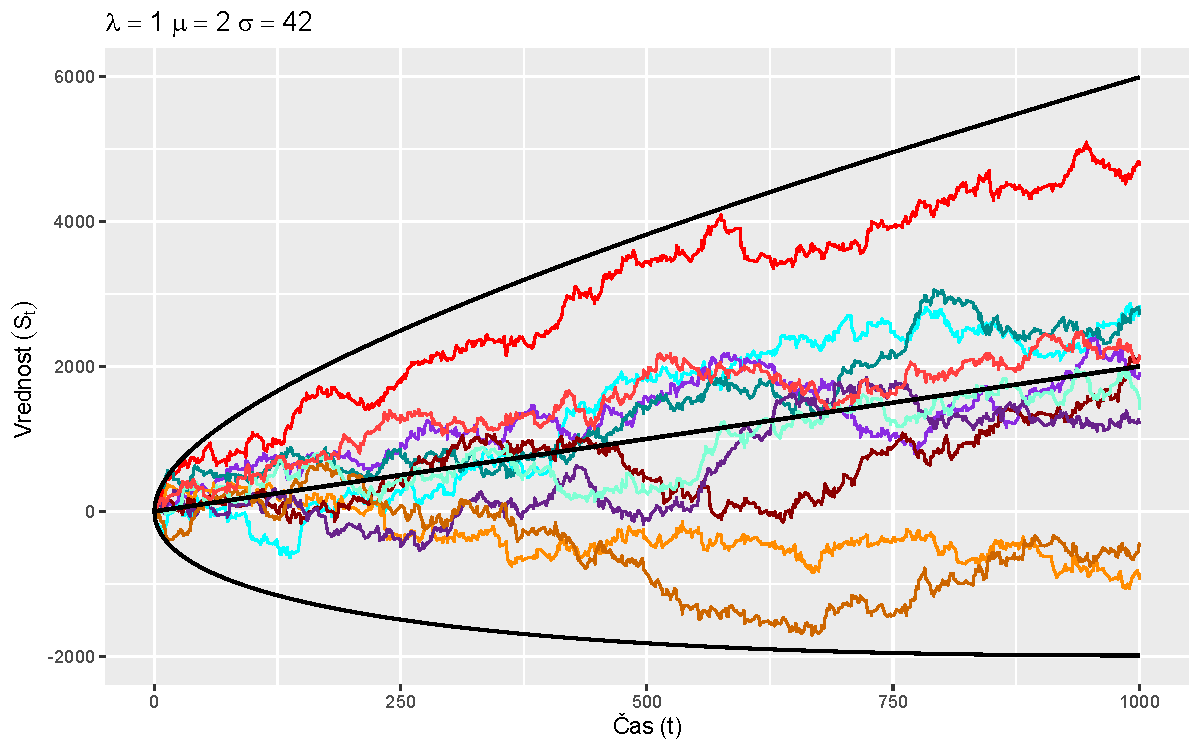
\includegraphics[width=0.8\textwidth]{
        C:/Users/38651/OneDrive - Univerza v Ljubljani/Desktop/Diploma/Diplomski-seminar/GraphsAndPhotos/slika6.pdf
        }
    \caption{Trajektorije CPP s funkcijami $t \mapsto \E\left[S_t\right]$ in $t \mapsto \E\left[S_t\right] \pm 3\sigma_{S_t}$}
    \label{fig:slika1}
\end{figure}
\end{frame}

%-----------------------------------------FRAME --------------------------------------------------%
\begin{frame}
  \frametitle{Cramér--Lundbergov model}
  \begin{definicija}
    Naj bo $(S_t)_{t\geq0 }$ $\CPP$, kjer so slu"cajne spremenljivke $(X_i)_{i\in\N}$, 
    ki jih se"stevamo skoraj gotovo nenegativne.\ \textit{Proces tveganja} v Cramér--Lundbergovem 
    modelu definiramo kot dru"zino slu"cajnih spremenljivk 
    \begin{align*}
        U_t = u + p(t) - S_t, \quad t\geq0,
    \end{align*}
    kjer je $u \geq 0$ za"cetni kapital zavarovalnice in $p$ funkcija prihodkov iz premij. 
    \label{def:procesTveganja}
  \end{definicija}
  \pause
  \begin{zgled}
    Naj bo $(U_t)_{t\geq0}$ proces tveganja v Cramér--Lundbergovem modelu z za"cetnim kapitalom
    $u = 1000$ in $p(t) = 200t$ ter intenzivnostjo prihodov zahtevkov $\lambda=1$. % v $CPP$. 
    Naj bodo v prvem primeru (rde"ca) 
    zahtevki porazdeljeni kot $X_i \sim \text{Weibull}(2, 434)$ in v drugem primeru (modra) kot
    $Y_i \sim \text{Weibull}(\tfrac{1}{4}, 16)$.
  \end{zgled}
\end{frame}

%-----------------------------------------FRAME --------------------------------------------------%
\begin{frame}
  \frametitle{Cramér--Lundbergov model}
  \begin{figure}[H]
    \centering
    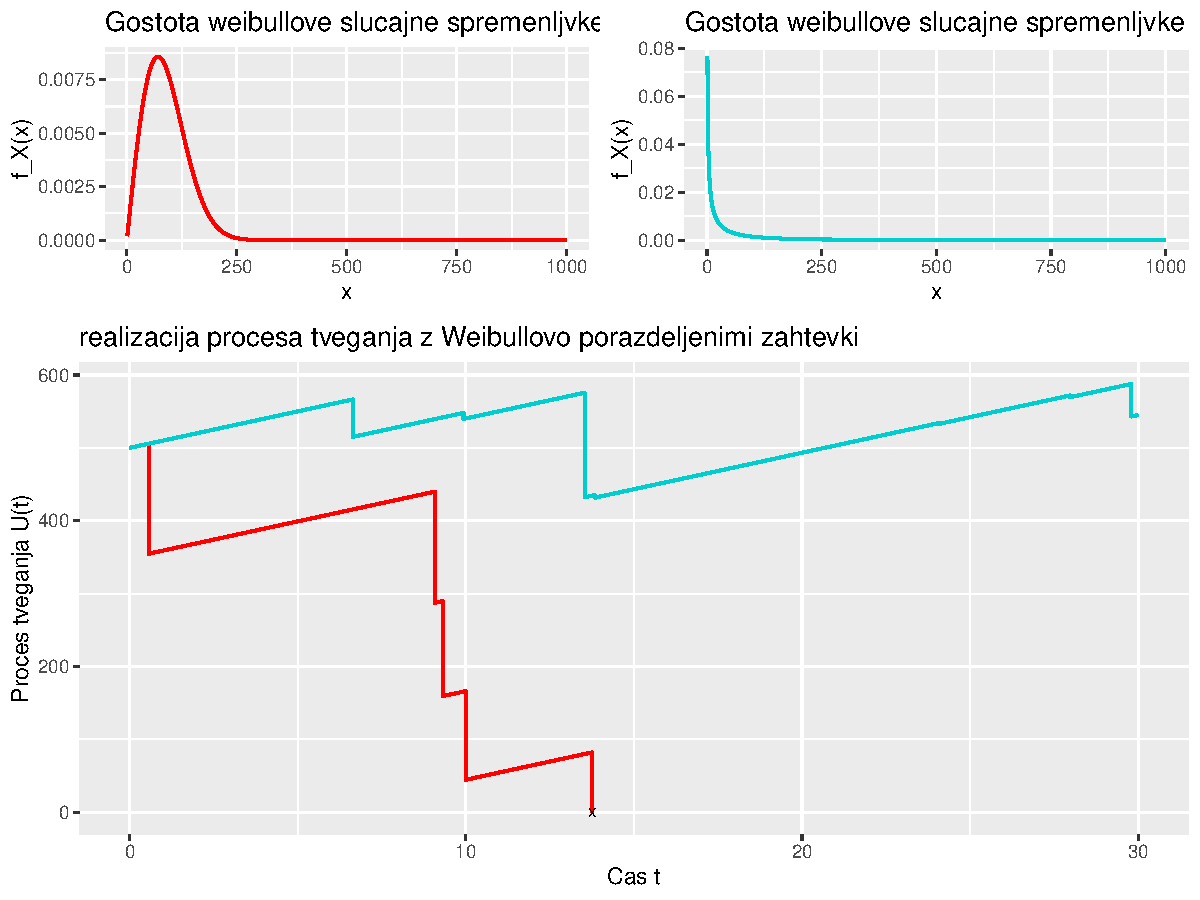
\includegraphics[width=0.7\textwidth]{
        C:/Users/38651/OneDrive - Univerza v Ljubljani/Desktop/Diploma/Diplomski-seminar/GraphsAndPhotos/slika2.pdf
        }
    \label{fig:slika2}
    \caption{Realizaciji procesa tveganja $U_t$ v Cramér--Lundbergovem modelu}
\end{figure}
\end{frame}

%-----------------------------------------FRAME --------------------------------------------------%
\begin{frame}
  \frametitle{Verjetnost propada}
  \begin{definicija}
    \textit{Propad} definiramo kot dogodek, da proces tveganja $(U_t)_{t\geq0}$ kadarkoli pade pod $0$. 
    To je torej dogodek 
    \begin{align*}
        \bigl\{U_t<0 \ \text{za neki} \ t\geq 0\bigr\}.
    \end{align*}
    "Casu ustavljanja
    \begin{align*}
        T = \inf\{t\geq0 \mid U_t < 0\}
    \end{align*}
    pa pravimo \textit{"cas propada}.
  \end{definicija}
  \pause
  \begin{definicija}
      \textit{Verjetnost propada} definiramo kot funkcijo $\psi: (0,\infty) \to [0,1]$ 
      s predpisom
      \begin{align*}
          \psi(u) = \Prob_u(T<\infty); \quad u\geq0.
      \end{align*}
  \end{definicija}
\end{frame}

%-----------------------------------------FRAME --------------------------------------------------%
\begin{frame}
  \frametitle{Prevedba na diskretni slu"cajni sprehod}
  \begin{definicija}
    Po konstrukciji procesa tveganja $(U_t)_{t\geq0}$ je propad mogo"c le ob 
    prihodih zahtevkov. %, ki sledijo $HPP(\lambda)$
    Z $V_n$ ozna"cimo "cas, ob katerem prispe $n$-ti zahtevek, in definiramo 
    \textit{ogrodje procesa tveganja} kot $(U_{V_n})_{n\in\N}$.
    \label{def:ogrodjeProcesaTveganja}
  \end{definicija}
  \pause
  \begin{trditev}
    Naj bo $(U_t)_{t\geq0}$ proces tveganja v Cramér--Lundbergovem modelu in $(U_{V_n})_{n\in\N}$ 
    njegovo ogrodje ter $T_n := V_n - V_{n-1}$ medprihodni "cas $n$-tega zahtevka 
    $(V_0 = T_0 = 0)$. Potem velja 
    \begin{equation*}
        \psi(u) = \Prob\left(\sup_{n\in\N}Z_n > u\right),
    \end{equation*}
    kjer je $Z_n = \sum_{i=1}^nY_i$  kumulativna izguba po $n$ zahtevkih in $Y_i = X_i - cT_i$
    izguba $i$-tega prihoda.
    \label{trd:verjetnostPropadaZOgrodjem}
  \end{trditev}
\end{frame}

%-----------------------------------------FRAME --------------------------------------------------%
\begin{frame}
  \frametitle{Pogoj neto zaslu"zka (NPC)}
  \begin{equation*}
    \E\left[Y_1\right] = \E\left[X_1\right] - c\E\left[T_1\right]
  \end{equation*}
  \begin{definicija}
    Pravimo, da proces tveganja $(U_t)_{t\geq0}$ v Cramér--Lundbergovem modelu
     zado"s"ca \textit{pogoju neto zaslu"zka} (ang. \textit{net profit condition}), "ce velja 
    \begin{equation*}
        c > \frac{\E\left[X_1\right]}{\E\left[T_1\right]}, \quad \text{oziroma} \quad 
        c = (1 + \rho)\frac{\E\left[X_1\right]}{\E\left[T_1\right]} \quad \text{za $\rho > 0$}.
    \end{equation*}
    Pogoj bomo v nadaljevanju imenovali NPC.
    \label{def:NPC}
  \end{definicija}
\end{frame}

%-----------------------------------------FRAME --------------------------------------------------%
\begin{frame}
  \frametitle{Verjetnost pre"zivetja}
  \begin{definicija}
    Za lep"so notacijo v nadaljevanju definiramo "se funkcijo \textit{verjetnosti pre"zivetja} kot
    $\theta:(0, \infty) \to [0, 1]$ s predpisom
    \begin{equation*}
        \theta(u) = \Prob_u\left(T=\infty\right) = 1 - \psi(u); \quad u\geq 0.
    \end{equation*}
    \label{def:verjetnostPrezivetja}
  \end{definicija}
  \pause
  \begin{lema}[Integralska ena"cba za verjetnost pre"zivetja]
    Naj bo $(U_t)_{t\geq0}$ proces tveganja v Cramér--Lundbergovem modelu, ki zado"s"ca NPC, ter naj 
    velja $\E\left[X_1\right]<\infty$ in da imajo slu"cajne spremenljivke $(X_i)_{i\in\N}$ 
    gostoto. Potem $\theta$ zado"s"ca  enakosti
    \begin{equation*}
        \theta(u) = \theta(0) + \frac{1}{(1+\rho)} \int_{(0, u]}\theta(u - x)d\overline{F}_{X_1}(x),
    \end{equation*}
    kjer je $\overline{F}_{X_1}$ porazdelitev integriranega repa  
    slu"cajne spremenljivke $X_1$.
    \label{lema:verjetnostPrezivetja}
  \end{lema}
\end{frame}

%-----------------------------------------FRAME --------------------------------------------------%
\begin{frame}
  \frametitle{Defektna prenovitvena ena"cba}
  \begin{equation*}
    \theta(u) = (1 - q) + q\int_{(0, u]}\theta(u - x)d\overline{F}_{X_1}(x).
  \end{equation*}
  \pause
  \begin{equation*}
    Ag(u) = (1 - q) + q\int_{(0, u]}g(u - x)d\overline{F}_{X_1}(x),
    \label{eq:operator}
  \end{equation*}
  \pause
  $A$ je skr"citev na prostoru omejenih funkcij $B([0, \infty))$, opremljene s supremum metriko
  \begin{equation*}
    d_\infty(f, g) = \sup_{u\in[0, \infty)}\big|f(u) - g(u)\big|,  \quad f, g\in B([0, \infty)).
  \end{equation*}
  \pause
  Izka"ze se, da z ustrezno izbiro funkcije $g_0\in B([0, \infty))$ lahko poka"zemo, da je 
  \begin{equation*}
    \theta(u) = \lim_{n\to\infty} A^ng_0 = (1 - q)\sum_{k = 0}^\infty q^k\Prob\left(\overline{W}_k \leq u\right).
  \end{equation*}
\end{frame}

%-----------------------------------------FRAME --------------------------------------------------%
\begin{frame}
  \frametitle{Lahkorepe porazdelitve}
  \begin{definicija}
    Naj velja, da ima slu"cajna spremenljivka $Y_1 = X_1 - cT_1$ iz trditve \ref{trd:verjetnostPropadaZOgrodjem} 
    lahek rep. "Ce obstaja enoli"cen $\ell > 0$, za katerega velja
    \begin{equation*}
        M_{Y_1}(\ell)  = 1,
    \end{equation*}
    temu "stevilu pravimo \textit{Lundbergov koeficient}.
    \label{def:LundbergovKoeficient}
  \end{definicija}
  \pause
  \begin{izrek}[Lundbergova neenakost]
    Naj bo $(U_t)_{t\geq0}$ proces tveganja v Cramér--Lundbergovem modelu, ki zado"s"ca pogoju NPC in 
     zanj obstaja Lundbergov koeficient $\ell$. Potem za vsak $u>0$ velja
    \begin{equation*}
        \psi(u) \leq e^{-\ell u}.
    \end{equation*}
    \label{izr:LundbergovaNeenakost}
  \end{izrek}
\end{frame}

%-----------------------------------------FRAME --------------------------------------------------%
\begin{frame}
  \frametitle{Lahkorepe porazdelitve}
  \begin{izrek}[Asimptotika verjetnosti propada, lahkorepe porazdelitve]
    Naj bo $(U_t)_{t\geq0}$ proces tveganja v Cramér--Lundbergovem modelu, ki zado"s"ca NPC in 
    naj zanj obstaja Lundbergov koeficient $\ell$. Naj imajo slu"cajne spremenljivke 
    $(X_i)_{i\in\N}$ gostoto.\ Potem obstaja konstanta $C>0$, za katero velja 
    \begin{equation*}
        \lim_{u\to\infty}e^{\ell u}\psi(u) = C.
    \end{equation*}
    \label{izr:CramerjevaMeja}
\end{izrek}
\pause
\begin{zgled}
  V primeru ko zahtevke $X_1, X_2, \dots$ modeliramo z eksponentno porazdelitvijo, torej $X_i\sim\text{Exp}(\mu)$,
  lahko eksplicitno izra"cunamo verjetnost propada
  \begin{equation*}
    \psi(u) =  \frac{1}{1+\rho}\,e^{-\ell u}.
    \label{eq:eksplicitnaVerjetnostPropadaExp}
\end{equation*}
\end{zgled}
\end{frame}

%-----------------------------------------FRAME --------------------------------------------------%
\begin{frame}
  \frametitle{Lahkorepe porazdelitve}
  \begin{figure}[H]
    \centering
    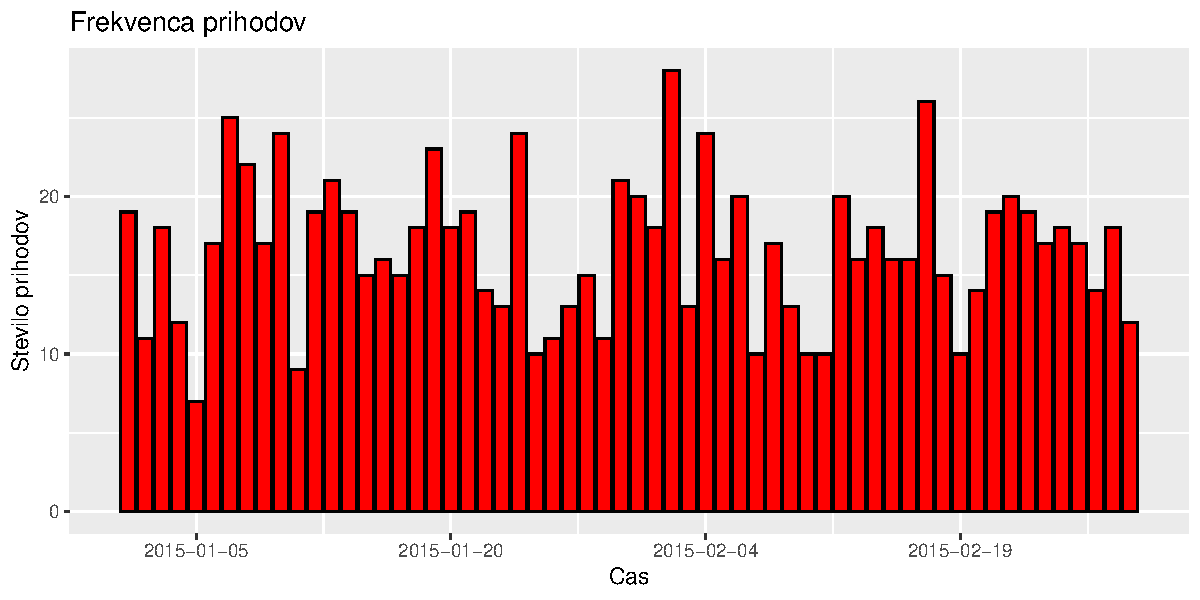
\includegraphics[width=0.8\textwidth]{
        C:/Users/38651/OneDrive - Univerza v Ljubljani/Desktop/Diploma/Diplomski-seminar/GraphsAndPhotos/slika3.pdf
        }
    \caption{Aproksimacija verjetnosti propada $\psi(u)$ z Monte Carlo simulacijami.}
    \label{fig:slika4}
\end{figure}
\end{frame}

%-----------------------------------------FRAME --------------------------------------------------%
\begin{frame}
  \frametitle{Subeksponentne porazdelitve}
  \begin{definicija}
    Verjetnostna porazdelitev $F$ na $[0, \infty)$ je \textit{subeksponentna}, "ce za vsak $n\geq2$ in 
    neodvisne slu"cajne spremenljivke $X_1, \dots, X_n$ s to porazdelitvijo velja 
    \begin{equation*}
        \lim_{x\to\infty}\frac{\Prob\left(X_1 + \cdots + X_n > x\right)}{\Prob\left(X_1 > x\right)} = n
    \end{equation*}
    in $F(x) < 1$ za vsak $x > 0$.
    \label{def:subeksponentnaPorazdelitev}
  \end{definicija}
\end{frame}

%-----------------------------------------FRAME --------------------------------------------------%
\begin{frame}
  \begin{izrek}[Asimptotika verjetnosti propada, subeksponentne porazdelitve]
    Naj bo $(U_t)_{t\geq0}$ proces tveganja v Cramér--Lundbergovem modelu, ki zado"s"ca NPC in 
    naj bodo zahtevki $(X_i)_{i\in\N}$ neodvisni in enako porazdeljeni z gostoto, 
    pri"cakovano vrednostjo $\E\left[X\right] < \infty$ in naj bo $\overline{F}_{X_1}$ subeksponentna.
    Potem za verjetnost propada $\psi(u)$ velja
    \begin{equation*}
        \lim_{u\to\infty}\frac{\psi(u)}{1 - \overline{F}_{X_1}(u)} = \frac{1}{\rho}.
        \label{eq:tezkorepnePorazdelitveAsimptotika}
    \end{equation*}
    \label{izr:tezkorepnePorazdelitveAsimptotika}
  \end{izrek}
\end{frame}






\end{document}

